% questions.tex —— 2005 年·上海卷·文科 · 题目内容片段（无答案）
% 由 tools/generate_projects.py 依来源总账自 2005/2005_数学真题_上海文_试题.md 生成，勿手改（改源 MD 后重跑）


\gkpart{数学试卷}

\begin{gktip}
\textbf{来源说明}：依据固定来源 PDF 原页转录。题签、题号、公式、选项和图位已对照 PDF 第 1–2 页及印刷页 264–265 目视核查；出版者、版次、复制链及官方身份未核。固定 PDF 只含题面页，没有答案页；本稿只记录题面。

\textbf{图表说明}：第 12、17、21 题图均依据固定原页可见关系矢量重绘；图稿链接位于对应题目下方。
\end{gktip}

\gkpart{一、填空题}

\begin{question}
\gkti{1}函数 $f(x)=\log_4(x+1)$ 的反函数 $f^{-1}(x)=\underline{\qquad}$。

\end{question}
\begin{question}
\gkti{2}方程 $4^x+2^x-2=0$ 的解是 $\underline{\qquad}$。

\end{question}
\begin{question}
\gkti{3}若 $x,y$ 满足条件 $\begin{cases}x+y\le 3,\\y\le 2x,\end{cases}$ 则 $z=3x+4y$ 的最大值是 $\underline{\qquad}$。

\end{question}
\begin{question}
\gkti{4}直角坐标平面 $xOy$ 中，若定点 $A(1,2)$ 与动点 $P(x,y)$ 满足 $\overrightarrow{OP}\cdot\overrightarrow{OA}=4$，则点 $P$ 的轨迹方程是 $\underline{\qquad}$。

\end{question}
\begin{question}
\gkti{5}函数 $y=\cos 2x+\sin x\cos x$ 的最小正周期 $T=\underline{\qquad}$。

\end{question}
\begin{question}
\gkti{6}若 $\cos\alpha=\frac17$，$\alpha\in\left(0,\frac\pi2\right)$，则 $\cos\left(\alpha+\frac\pi3\right)=\underline{\qquad}$。

\end{question}
\begin{question}
\gkti{7}若椭圆长轴长与短轴长之比为 $2$，它的一个焦点是 $(2\sqrt{15},0)$，则椭圆的标准方程是 $\underline{\qquad}$。

\end{question}
\begin{question}
\gkti{8}某班有 $50$ 名学生，其中 $15$ 人选修 $A$ 课程，另外 $35$ 人选修 $B$ 课程。从班级中任选两名学生，他们是选修不同课程的学生的概率是 $\underline{\qquad}$。（结果用分数表示。）

\end{question}
\begin{question}
\gkti{9}直线 $y=\frac12x$ 关于直线 $x=1$ 对称的直线方程是 $\underline{\qquad}$。

\end{question}
\begin{question}
\gkti{10}在 $\triangle ABC$ 中，若 $A=120^\circ$，$AB=5$，$BC=7$，则 $AC=\underline{\qquad}$。

\end{question}
\begin{question}
\gkti{11}函数 $f(x)=\sin x+2|\sin x|$，$x\in[0,2\pi]$ 的图象与直线 $y=k$ 有且仅有两个不同的交点，则 $k$ 的取值范围是 $\underline{\qquad}$。

\Needspace{0.4\textheight}
\end{question}
\begin{question}
\gkti{12}有两个相同的直三棱柱，高为 $\frac2a$，底面三角形的三边长分别为 $3a,4a,5a$（$a>0$）。用它们拼成一个三棱柱或四棱柱，在所有可能的情形中，全面积最小的是一个四棱柱，则 $a$ 的取值范围是 $\underline{\qquad}$。
\nopagebreak[4]
\begin{center}% 2005 年上海文科卷第 12 题：两个拼合示意
\begin{tikzpicture}[scale=0.78]
  % 原页并排重复的两幅棱柱拼合示意；尺寸标注不代表绘图比例。
  \foreach \dx in {0,5} {
    \begin{scope}[shift={ (\dx,0) }]
      \coordinate (A) at (0,0);
      \coordinate (B) at (3.15,0);
      \coordinate (C) at (3.15,1.05);
      \coordinate (D) at (0,1.05);
      \coordinate (E) at (2.10,1.62);
      \coordinate (F) at (2.10,0.57);

      % 可见棱与隐藏棱
      \draw (A)--(B)--(C)--(D)--(E)--(C);
      \draw (D)--(A);
      \draw[dashed] (E)--(F);
      \draw[dashed] (A)--(F)--(B);

      % 尺寸标注
      \node[left] at (-0.15,0.53) {$\dfrac{2}{a}$};
      \node[below] at (1.58,-0.18) {$5a$};
      \node[below,rotate=-29] at (2.65,0.24) {$3a$};
      \node[above,rotate=15] at (1.12,0.23) {$4a$};
    \end{scope}
  }
\end{tikzpicture}
\end{center}
\nopagebreak[4]
\begin{gktip}
固定原页的两幅图线形重复，按原样重复转绘；不据此分别标注拼合类型。
\end{gktip}

\end{question}
\gkpart{二、选择题}

\begin{question}
\gkti{13}若函数 $f(x)=\dfrac{1}{2^x+1}$，则该函数在 $(-\infty,+\infty)$ 上是\mbox{（　　）}。

（A）单调递减无最小值　　（B）单调递减有最小值

（C）单调递增无最大值　　（D）单调递增有最大值

\end{question}
\begin{question}
\gkti{14}已知集合 $M=\{x\mid |x-1|\le 2,\ x\in\mathbb R\}$，$P=\left\{x\mid \dfrac{5}{x+1}\ge 1,\ x\in\mathbb Z\right\}$，则 $M\cap P$ 等于\mbox{（　　）}。

（A）$\{x\mid 0<x\le 3,\ x\in\mathbb Z\}$　　（B）$\{x\mid 0\le x\le 3,\ x\in\mathbb Z\}$

（C）$\{x\mid -1\le x\le 0,\ x\in\mathbb Z\}$　　（D）$\{x\mid -1\le x<0,\ x\in\mathbb Z\}$

\end{question}
\begin{question}
\gkti{15}条件甲：“$a>1$”是条件乙：“$a>\sqrt a$”的\mbox{（　　）}。

（A）既不充分也不必要条件　　（B）充要条件

（C）充分不必要条件　　（D）必要不充分条件

\end{question}
\begin{question}
\gkti{16}用 $n$ 个不同的实数 $a_1,a_2,\ldots,a_n$ 可得到 $n!$ 个不同的排列，每个排列为一行写成一个 $n!$ 行的数阵。对第 $i$ 行 $a_{i1},a_{i2},\ldots,a_{in}$，记

\nopagebreak[4]
\[b_i=-a_{i1}+2a_{i2}-3a_{i3}+\cdots+(-1)^n n a_{in},\qquad i=1,2,3,\ldots,n!.\]

\Needspace{5\baselineskip}
例如：用 $1,2,3$ 可得数阵如下。由于此数阵中每一列各数之和都是 $12$，所以，

\nopagebreak[4]
\[b_1+b_2+\cdots+b_6=-12+2\times12-3\times12=-24.\]

\Needspace{5\baselineskip}
那么，在用 $1,2,3,4,5$ 形成的数阵中，$b_1+b_2+\cdots+b_{120}=$\mbox{（　　）}。

\nopagebreak[4]
\[\begin{array}{ccc}
1&2&3\\
1&3&2\\
2&1&3\\
2&3&1\\
3&1&2\\
3&2&1
\end{array}\]

（A）$-3600$　　（B）$1800$　　（C）$-1080$　　（D）$-720$

\end{question}
\gkpart{三、解答题}

\Needspace{0.4\textheight}
\begin{question}
\gkti{17}已知长方体 $ABCD-A_1B_1C_1D_1$ 中，$M,N$ 分别是 $BB_1$ 和 $BC$ 的中点，$AB=4$，$AD=2$，$B_1D$ 与平面 $ABCD$ 所成角的大小为 $60^\circ$，求异面直线 $B_1D$ 与 $MN$ 所成角的大小。（结果用反三角函数值表示。）
\nopagebreak[4]
\begin{center}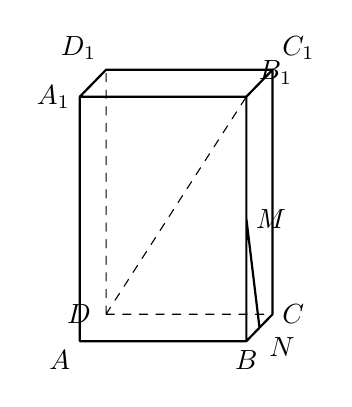
\begin{tikzpicture}[line cap=round,line join=round,x=0.9cm,y=0.9cm]
  \coordinate (A) at (0,0);
  \coordinate (B) at (2.35,0);
  \coordinate (C) at (2.72,0.38);
  \coordinate (D) at (0.37,0.38);
  \coordinate (Aone) at (0,3.45);
  \coordinate (Bone) at (2.35,3.45);
  \coordinate (Cone) at (2.72,3.83);
  \coordinate (Done) at (0.37,3.83);
  \coordinate (M) at (2.35,1.725);
  \coordinate (N) at (2.535,0.19);

  % Rear-left and rear-bottom edges are hidden; B_1D is hidden inside the prism.
  \draw[dashed] (D)--(C) (D)--(Done) (D)--(Bone);
  \draw[thick] (A)--(B)--(C) (A)--(Aone)--(Bone)--(Cone)--(Done)--(Aone)
               (B)--(Bone) (C)--(Cone) (M)--(N);

  \node[below left] at (A) {$A$};
  \node[below] at (B) {$B$};
  \node[right] at (C) {$C$};
  \node[left=2pt] at (D) {$D$};
  \node[left] at (Aone) {$A_1$};
  \node[above right=1pt] at (Bone) {$B_1$};
  \node[above right] at (Cone) {$C_1$};
  \node[above left] at (Done) {$D_1$};
  \node[right] at (M) {$M$};
  \node[below right] at (N) {$N$};
\end{tikzpicture}
\end{center}
\nopagebreak[4]
\end{question}
\begin{question}
\gkti{18}在复数范围内解方程 $|z|^2+(z+\overline z)i=\dfrac{3-i}{2+i}$。（$i$ 为虚数单位。）

\end{question}
\begin{question}
\gkti{19}已知函数 $f(x)=kx+b$ 的图象与 $x,y$ 轴分别相交于点 $A,B$，$\overrightarrow{AB}=2\vec i+2\vec j$（$\vec i,\vec j$ 分别是与 $x,y$ 轴正半轴同方向的单位向量），函数 $g(x)=x^2-x-6$。

（1） 求 $k,b$ 的值；

（2） 当 $x$ 满足 $f(x)>g(x)$ 时，求函数 $\dfrac{g(x)+1}{f(x)}$ 的最小值。

\end{question}
\begin{question}
\gkti{20}假设某市 $2004$ 年新建住房面积 $400$ 万平方米，其中有 $250$ 万平方米是中低价房。预计在今后的若干年内，该市每年新建住房面积平均比上一年增长 $8\%$。另外，每年新建住房中，中低价房的面积均比上一年增加 $50$ 万平方米。那么，到哪一年底，

（1） 该市历年所建中低价层的累计面积（以 $2004$ 年为累计的第一年）将首次不少于 $4750$ 万平方米？

（2） 当年建造的中低价房的面积占该年建造住房面积的比例首次大于 $85\%$？

\begin{gktip}
原件在第（1）问印作“中低价层”，与本题前文及第（2）问的“中低价房”不一致；此处照录原字样，未擅自改写。
\end{gktip}

\Needspace{0.4\textheight}
\end{question}
\begin{question}
\gkti{21}已知抛物线 $y^2=2px$（$p>0$）的焦点为 $F$，$A$ 是抛物线上横坐标为 $4$、且位于 $x$ 轴上方的点，$A$ 到抛物线准线的距离等于 $5$。过 $A$ 作 $AB$ 垂直于 $y$ 轴，垂足为 $B$，$OB$ 的中点为 $M$。

（1） 求抛物线方程；

（2） 过 $M$ 作 $MN\perp FA$，垂足为 $N$，求点 $N$ 的坐标；

（3） 以 $M$ 为圆心，$MB$ 为半径作圆 $M$，当 $K(m,0)$ 是 $x$ 轴上一动点时，讨论直线 $AK$ 与圆 $M$ 的位置关系。
\nopagebreak[4]
\begin{center}% 2005 年上海卷文科普通卷第 21 题：抛物线、焦点及垂线关系示意（不按比例）。
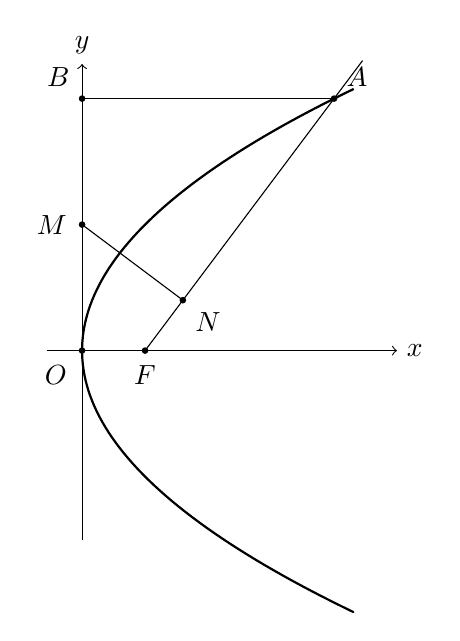
\begin{tikzpicture}[x=0.8cm,y=0.8cm,line cap=round,line join=round]
  % 以 y^2=4x 仅作形状示意；题面未给出 p 的数值。
  \draw[->] (-0.55,0)--(5.0,0) node[right] {$x$};
  \draw[->] (0,-3.0)--(0,4.55) node[above] {$y$};
  \draw[thick,domain=-4.15:4.15,samples=100] plot ({\x*\x/4},{\x});

  % A=(4,4), F=(1,0), B=(0,4), M 为 OB 中点；N 为 M 到 FA 的垂足。
  \draw (0,4)--(4,4);
  \draw (1,0)--(4.45,4.6);
  \draw (0,2)--(1.6,0.8);

  \fill (0,0) circle (1.2pt) node[below left=2pt] {$O$};
  \fill (1,0) circle (1.2pt) node[below=2pt] {$F$};
  \fill (4,4) circle (1.2pt) node[above right=1pt] {$A$};
  \fill (0,4) circle (1.2pt) node[above left=1pt] {$B$};
  \fill (0,2) circle (1.2pt) node[left=2pt] {$M$};
  \fill (1.6,0.8) circle (1.2pt) node[below right=1pt] {$N$};
\end{tikzpicture}
\end{center}
\nopagebreak[4]
\end{question}
\begin{question}
\gkti{22}对定义域是 $D_f,D_g$ 的函数 $y=f(x),y=g(x)$，规定函数 $h(x)$ 为

\nopagebreak[4]
\[h(x)=\begin{cases}
f(x)g(x),&x\in D_f\text{ \text{且} }x\in D_g,\\
f(x),&x\in D_f\text{ \text{且} }x\notin D_g,\\
g(x),&x\notin D_f\text{ \text{且} }x\in D_g.
\end{cases}\]

（1） 若函数 $f(x)=-2x+3$，$x\ge 1$，$g(x)=x-2$，$x\in\mathbb R$，写出函数 $h(x)$ 的解析式；

（2） 求问题（1）中函数 $h(x)$ 的最大值；

（3） 若 $g(x)=f(x+\alpha)$，其中 $\alpha$ 是常数，且 $\alpha\in[0,\pi]$，请设计一个定义域为 $\mathbb R$ 的函数 $y=f(x)$，及一个 $\alpha$ 的值，使得 $h(x)=\cos 4x$，并予以证明。

\end{question}